\section{Jeu de la vie} % (fold)
\label{sec:jeu_de_la_vie}

Le jeu de la vie est un modèle d'automate, dans lequel chacun des états connaît son état futur par le calcul de règles préétablies. Le jeu a été imaginé sur une grille à deux dimensions mais pourrait se généraliser dans n'importe quelle dimension. Nous allons toujours parler du jeu en deux dimensions. Les règles du jeu de la vie, pour chaque cellule, sont dépendantes des huit cellules voisines.
\begin{itemize}
\item Une cellule morte possédant exactement trois voisines vivantes devient vivante.
\item Une cellule vivante possédant deux ou trois voisines vivantes le reste, sinon elle meurt.
\end{itemize}

Ainsi, lorsque l'on possède trois voisins, nous sommes donc assurés d'être vivants (Fig. \ref{alive}), deux voisins signifient que l'on reste dans le même état (Fig. \ref{nochange}), et strictement moins de deux ou strictement plus de trois nous font mourir (Fig. \ref{dead}).

\begin{figure}[h!]
\centering
\begin{minipage}{.3\textwidth}
\centering
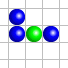
\includegraphics[width=0.5\textwidth]{Gol-born}
\caption{Une cellule vit}
\label{alive}
\end{minipage}
\hspace{0.5cm}
\begin{minipage}{0.3\textwidth}
\centering
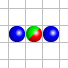
\includegraphics[width=0.5\textwidth]{Gol-nochange}
\caption{Conservation d'un état}
\label{nochange}
\end{minipage}
\hspace{0.5cm}
\begin{minipage}{.3\textwidth}
\centering
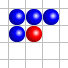
\includegraphics[width=0.5\textwidth]{Gol-dead}
\caption{Une cellule meurt}
\label{dead}
\end{minipage}
\end{figure}


A partir de cet énoncé, une version séquentielle du jeu de la vie a été fabriquée. 